% THIS IS SIGPROC-SP.TEX - VERSION 3.1
% WORKS WITH V3.2SP OF ACM_PROC_ARTICLE-SP.CLS
% APRIL 2009
%
% It is an example file showing how to use the 'acm_proc_article-sp.cls' V3.2SP
% LaTeX2e document class file for Conference Proceedings submissions.
% ----------------------------------------------------------------------------------------------------------------
% This .tex file (and associated .cls V3.2SP) *DOES NOT* produce:
%       1) The Permission Statement
%       2) The Conference (location) Info information
%       3) The Copyright Line with ACM data
%       4) Page numbering
% ---------------------------------------------------------------------------------------------------------------
% It is an example which *does* use the .bib file (from which the .bbl file
% is produced).
% REMEMBER HOWEVER: After having produced the .bbl file,
% and prior to final submission,
% you need to 'insert'  your .bbl file into your source .tex file so as to provide
% ONE 'self-contained' source file.
%
% Questions regarding SIGS should be sent to
% Adrienne Griscti ---> griscti@acm.org
%
% Questions/suggestions regarding the guidelines, .tex and .cls files, etc. to
% Gerald Murray ---> murray@hq.acm.org
%
% For tracking purposes - this is V3.1SP - APRIL 2009

\documentclass{acm_proc_article-sp}

\begin{document}

\title{Ramp it up! Action based guide for \\creating accessible websites\titlenote{A large format version of this poster is available at the author's website at \texttt{terracoda.net}}}
%
% You need the command \numberofauthors to handle the 'placement
% and alignment' of the authors beneath the title.
%
% For aesthetic reasons, we recommend 'three authors at a time'
% i.e. three 'name/affiliation blocks' be placed beneath the title.
%
% NOTE: You are NOT restricted in how many 'rows' of
% "name/affiliations" may appear. We just ask that you restrict
% the number of 'columns' to three.
%
% Because of the available 'opening page real-estate'
% we ask you to refrain from putting more than six authors
% (two rows with three columns) beneath the article title.
% More than six makes the first-page appear very cluttered indeed.
%
% Use the \alignauthor commands to handle the names
% and affiliations for an 'aesthetic maximum' of six authors.
% Add names, affiliations, addresses for
% the seventh etc. author(s) as the argument for the
% \additionalauthors command.
% These 'additional authors' will be output/set for you
% without further effort on your part as the last section in
% the body of your article BEFORE References or any Appendices.

\numberofauthors{1} %  in this sample file, there are a *total*
% of EIGHT authors. SIX appear on the 'first-page' (for formatting
% reasons) and the remaining two appear in the \additionalauthors section.
%
\author{
% You can go ahead and credit any number of authors here,
% e.g. one 'row of three' or two rows (consisting of one row of three
% and a second row of one, two or three).
%
% The command \alignauthor (no curly braces needed) should
% precede each author name, affiliation/snail-mail address and
% e-mail address. Additionally, tag each line of
% affiliation/address with \affaddr, and tag the
% e-mail address with \email.
%
% 1st. author
\alignauthor
Taliesin L. Smith\titlenote{The author is also an Instructional Design Specialist at Memorial University, St.John's, Newfoundland Labrador}\\
       \affaddr{MDes. (Candidate) Inclusive Design, }\affaddr{OCAD University, }\\
       \affaddr{Toronto, Ontario, Canada}\\
       \email{talilief@gmail.com}
}
\date{19 January 2015}

\maketitle
\begin{abstract}
Presented here is an action-based guide to create accessible websites. By focusing on accessibility rather than compliance this guide will help teams create sites that are perceivable, operable, understandable \& robust. The POUR principles of the Web Content Accessibility Guidelines (WCAG 2.0) are what all the other layers of guidance in the WCAG aim to achieve. The simplified techniques presented here focus on accessibile design decisions \& reframe the WCAG's layers into something all members of the web team - designers, developers, writers \& managers - can understand. To build in the \textit{virtual ramp} the entire team needs to be aware, develop the skill \& demand the necessary resources.

\end{abstract}

% A category with the (minimum) three required fields and an optionl 4th field 
% \category{H.1.2}{User/Machine Systems}{Human Factors}
%\category{D.2.8}{Software Engineering}{Metrics}[complexity measures, performance measures]
\category{H.1.2}{User/Machine Systems}{Human Factors}
\category{H.5.2}{User Interfaces}{Standardization}
\category{H.5.4}{Hypertext/ Hypermedia}{User issues}
\category{D.2.10}{Design}{Methodologies}

%\terms{web accessibility, WCAG, standards, inclusive design} % NOT required for Proceedings

\section{Introduction}
A long term study [4] found low compliance rates with the Web Content Accessibility Guidelines (WCAG), but at the same time, uncovered a growing adherence to \textit{some} criteria. A follow-up study [10] found that at least part of the improved accessibility was a side effect of changes in coding practices, new browser capabilities \& concerns over page rankings. In another study [8], \textit{lack of awareness \& knowledge of the WCAG} was identified by the participants to be the most significant barrier to web accessibility. These studies show that web teams continue to struggle with correct implementation of the WCAG \& suggest that aids that make the guidelines easier to understand could improve implementation. This poster intends to do just that, present the guidelines in a way that keeps team members focused on accessibility \& building in the \textit{virtual ramp}. 

\begin{figure*}
\centering
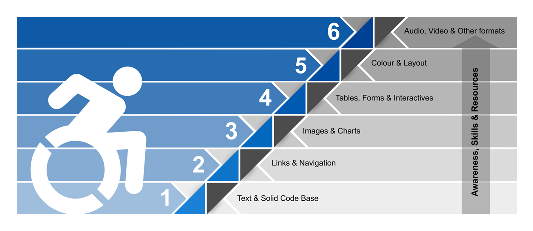
\epsfig{file=stairs-ramp.eps, width=14cm}
\caption{Each content type \& design decision is a potential barrier (stair). The numbers associate each stair with techniques for building in the \textit{virtual ramp}.}
\end{figure*}

\section{Building in the {\secit Virtual} Ramp}

\subsection{Text \& Solid Code Base}

Electronic text-based content is accessible by nature. It can be rendered visually, auditorily \& tactilely: Use HTML's built-in semantic structure [2,6] - headings, lists, quotes - to code meaning directly into your content. Keep the reading level as simple as possible. Define the natural language \& mark language changes. Ensure templates have a doctype, charset \& page title (a valid code base). Make page titles unique so users know they are in the right place.

\subsection{Navigation, Links \& Landmarks}
Navigation, links \& landmarks, like stepping stones, help you find your way [6]. Use unique self-describing meaningful words for linked text. Leave context changes - pop-ups, new tabs - in the control of the user. Use WAI-ARIA landmark roles [6], HTML5 landmark tags or skip-navigation links to provide direct access to page content. Design well-planned, consistent navigation to make sites accessible \& usable.

\subsection{Images \& Charts}
Provide meaningful text alternatives for all content images. The alt attribute is required, but can be left empty when appropriate. For charts or complex images you may need to link to supplementary content or use the longdesc attribute. The goal of text alternatives is to maintain the meaning of the document whether you can see the image or not.

\subsection{Tables, Forms \& Interactives}
For complex HTML structures, consider simplification whenever possible. For successful interaction the keyboard must be your guide.
\subsubsection{Table structure conveys meaning}
Use the rich semantic mark-up available for tables - caption, thead, tfoot, tbody - to make data realtionships clear. Appropriately distinguish table header cells from table data cells (th, td) on rows \& columns. Do not use tables for layout. They are for tabular data only!
\subsubsection{Forms \& Interactives are complex by nature}
Keep user control \& keyboard access top of mind. Use \& associate labels for every form control. Use the button element when you need a button. Exploit group form controls to create meaningful organization - legend, fieldset, optgroup. Organizational meaning is good for usability. Design clear error identification \& intuitive error handling by clearly telling the user where they have gone wrong, how to fix the problem \& when they have succeeded. Provide reasonable time-outs (think user control). Employ WAI-ARIA [6] to define roles \& behaviours that HTML cannot describe. This is particularly important for forms \& interactive structures that use forms.

Note: most legal cases have happened around inaccessible tables \& forms [9].

\subsection{Colour \& Layout}
CSS is the standard to use for presentation. Use it correctly to maintain global control of your layout \& design. Using CSS \& HTML together properly is best method in making your content accessible \& easier to maintain. Choose colours wisely \& test for sufficient contrast ratios. Avoid confusing colours [1]. Don't rely on colour alone for meaning.

\subsection{Audio, Video \& Other formats}
Like images multimedia need text alternatives to be made accessible. Provide captions for video \& transcripts for audio. For ultimate accessibilty describe video when the meaning cannot be understood by the soundtrack alone. Controls for media must be operable by the keyboard. Do not auto-play anything (think user control). For other formats, such as PDF or Word documents, first ask is there a reason not to use HTML? When HTML is not an option, follow the same principles (WCAG) discussed here to make content in documents accessible.

\section{Conclusions}
Creating websites that meet the needs of people with disabilities overlaps with people with situational limitations such as being in a loud environment, having limited use of hands, using a mobile device, using old hardware or having limited access to bandwidth [5]. Just as access ramps \& curbcuts benefit more than just people in wheelchairs, the \textit{virtual ramp} or \textit{electronic curbcut} [7] benefits more than just people using assitive technology. Making accessibility a priority in the design process helps us build better websites \& brings us closer to a universal web [5].
%\end{document}  % This is where a 'short' article might terminate

%ACKNOWLEDGMENTS are optional
\section{Acknowledgments}
Special thanks to the {\it Accessible Icon Project} \& Amita Pharshy.

%REFERENCES as a SECTION
\section{References}
\begin{itemize}
%\item[1] (2013) Semantic Structure. WebAIM.org. \\http://webaim.org/techniques/semanticstructure/
%\item[1] Don't reapeat yourself. Wikipedia.\\http://wikipedia.org/wiki/Don't\_repeat\_yourself
\item[1] Brewer, C., Harrower, M. \& Pennsylvania State University. {\it Color Brewer 2.0}. http://colorbrewer2.org/
\item[2] Clark, J. (2003). {\it Building accessible websites.} Indianapolis: New Riders.
%\item[6] Clark, J. (2005). Facts and opinions about PDF accessibility. {\it %A List Apart.}\\http://alistapart.com/article/pdf\_accessibility
\item[4] Hanson, V. \& Richards, J. (2013). Progress on website accessibility? {\it ACM Transactions on the Web, 7}(1). DOI:10.1145/2435215.2435217 
\item[5] Henry, S., Abou-Zahra, S., \& Brewer, J. (2014). The role of accessibility in a universal web. Paper presented at the {\it W4A - 11th Web for All 2014 Conference}. DOI:10.1145/2596695.2596719
\item[6] Horton, S. \& Quesenbery, W. (2014). {\it A Web for everyone: Designing accessible user experiences.} Brooklyn: Rosenfeld Media.
\item[7] Jacobs, S. (1999). Section 255 of the Telecommunications Act of 1996: Fueling the Creation of New Electronic Curbcuts. http://www.accessiblesociety.org/topics/\\technolog/eleccurbcut.htm 
\item[8] Lazar, J., Dudley-Sponaugle, A. \& Greenidge, K. (2004). Improving web accessibility: as study of web master perceptions. {\it Computers in Human Behavior, 20}(2). pp 269-288. DOI: 10.1016/j.chb.2003.10.018 
\item[9] Monsebraaten, L. (2012). Toronto woman wins second victory ordering governemnt websites accessible to the blind. {\it Toronto Star}. http://www.thestar.com/news/\\gta/2012/05/31/toronto\_woman\_wins\_second\_victory\_\\ordering\_government\_websites\_accessible\_to\_blind.html
\item[10] Richards, J., Montague, K. \& Hanson, V. (2012). Web Accessibility as a Side Effect, {\it ASSETS '12 Proceedings of the 14th International ACM SIGACCESS Conference on Computers \& Acessibility}. pp 79-86.
%\item[11] CSS. http://www.w3.org/TR/CSS
%\item[12] WAI-ARI. http://www.w3.org/TR/wai-aria
%\item[13] WCAG 2.0. http://www.w3.org/TR/WCAG20
%\item[14] WCAG Samurai: http://www.wcagsamurai.org
%\item[15] WCAG 1.0: http://www.w3.org/TR/WAI-WEBCONTENT		
\end{itemize}
%
% The following two commands are all you need in the
% initial runs of your .tex file to
% produce the bibliography for the citations in your paper.
\bibliographystyle{abbrv}
\bibliography{sigproc}  % sigproc.bib is the name of the Bibliography in this case
% You must have a proper ".bib" file
%  and remember to run:
% latex bibtex latex latex
% to resolve all references
%
% ACM needs 'a single self-contained file'!
%
\balancecolumns
% That's all folks!
\end{document}
